Depois de séculos de escaramuças entre os quatro povos habitantes da Nlogônia, e
de dezenas de anos de negociações envolvendo diplomatas, políticos e as forças
armadas de todas as partes interessadas, com a intermediação da ONU, OTAN, G7 e
SBC, foi finalmente decidida e aceita por todos a maneira de dividir o país em
quatro territórios independentes.

Ficou decidido que um ponto, denominado \textit{ponto divisor}, cujas
coordenadas foram estabelecidas nas negociações, definiria a divisão do país da
seguinte maneira.  Duas linhas, ambas contendo o ponto divisor, uma na direção
norte-sul e uma na direção leste-oeste, seriam traçadas no mapa, dividindo o
país em quatro novos países. Iniciando no quadrante mais ao norte e mais ao
oeste, em sentido horário, os novos países seriam chamados de Nlogônia do
Noroeste, Nlogônia do Nordeste, Nlogônia do Sudeste e Nlogônia do Sudoeste.

\begin{center}
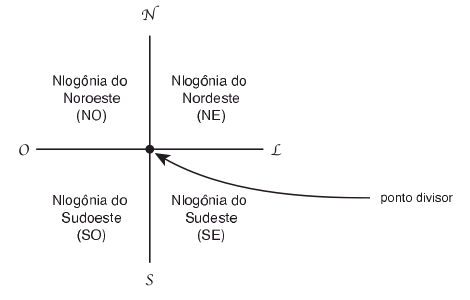
\includegraphics[scale=0.6]{problems/nlogonia/imagens/nlogonia.png}
\end{center}

A ONU determinou que fosse disponibilizada uma página na Internet para que os
habitantes pudessem consultar em qual dos novos países suas residências estão, e
você foi contratado para ajudar a implementar o sistema.

\subsection*{Entrada}

A entrada contém vários casos de teste. A primeira linha de um caso de teste
contém um inteiro $K$ indicando o número de consultas que serão realizadas
$(0 < K \leq 10^3)$. A segunda linha de um caso de teste contém dois números
inteiros $N$ e $M$ representando as coordenadas do ponto divisor
$(-10^4 < N, M < 10^4)$. Cada uma das $K$ linhas seguintes contém dois inteiros
$X$ e $Y$ representando as coordenadas de uma residência $(-10^4 \leq X, Y \leq 10^4)$.
Em todas as coordenadas dadas, o primeiro valor corresponde à direção leste-oeste, e o
segundo valor corresponde à direção norte-sul.

O final da entrada é indicado por uma linha que contém apenas o número zero.

\subsection*{Saída}


Para cada caso de teste da entrada seu programa deve imprimir uma linha
contendo:
\begin{itemize}
\item a palavra $divisa$ se a residência encontra-se em cima de uma das linhas
divisórias (norte-sul ou leste-oeste);

\item $NO$ se a residência encontra-se na Nlogônia do Noroeste;

\item $NE$ se a residência encontra-se na Nlogônia do Nordeste;

\item $SE$ se a residência encontra-se na Nlogônia do Sudeste;

\item $SO$ se a residência encontra-se na Nlogônia do Sudoeste.

\end{itemize}

\begin{table}[!h]
\centering
\begin{tabular}{|l|l|}
\hline
\begin{minipage}[t]{3in}
\textbf{Exemplo de entrada}
\begin{verbatim}
3
2 1
10 10
-10 1
0 33
4
-1000 -1000
-1000 -1000
0 0
-2000 -10000
-999 -1001
0
\end{verbatim}
\vspace{1mm}
\end{minipage}
&

\begin{minipage}[t]{3in}
\textbf{Exemplo de saída}
\begin{verbatim}
NE
divisa
NO
divisa
NE
SO
SE
\end{verbatim}
\vspace{1mm}
\end{minipage} \\
\hline
\end{tabular}
\end{table}

\newpage
